\subsubsection{\textbf{Wifi - Lan}}
Se hicieron prebas de ping Wifi - Lan con diferentes paquetes:

    \begin{figure}[H]
        \centering
        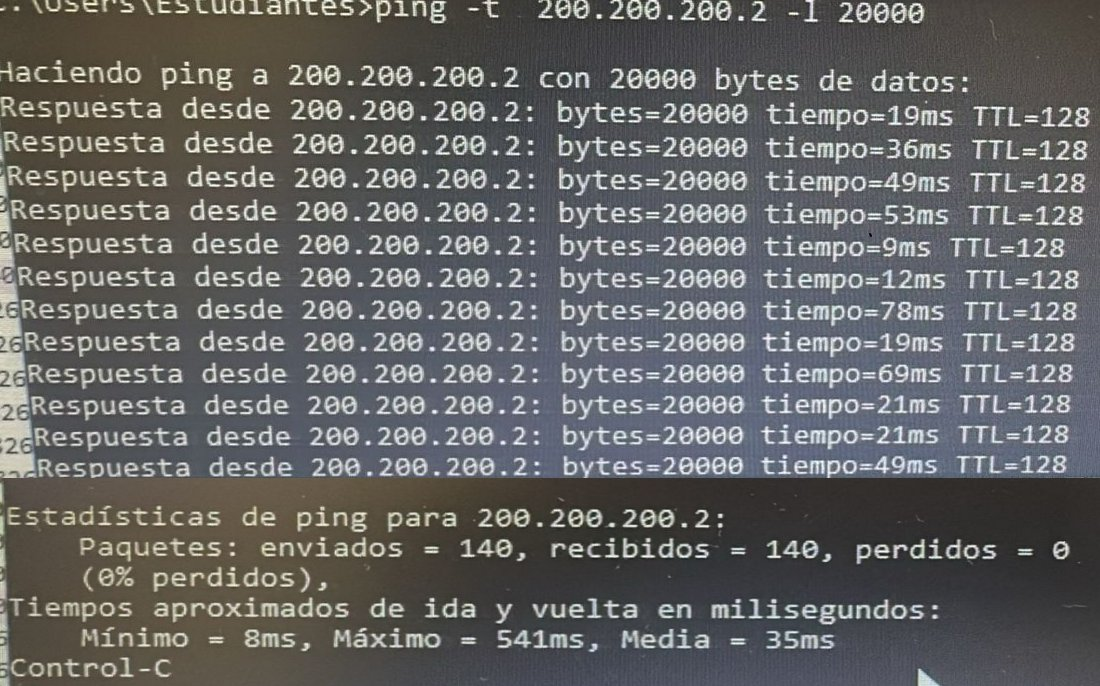
\includegraphics[width=\columnwidth]{punto1/p1_ping_wifi_lan_20k.jpeg}
        \caption{Ping Wifi - Lan, 20000}
        \label{fig:ping_wifi_lan_20k}
    \end{figure}

    \begin{figure}[H]
        \centering
        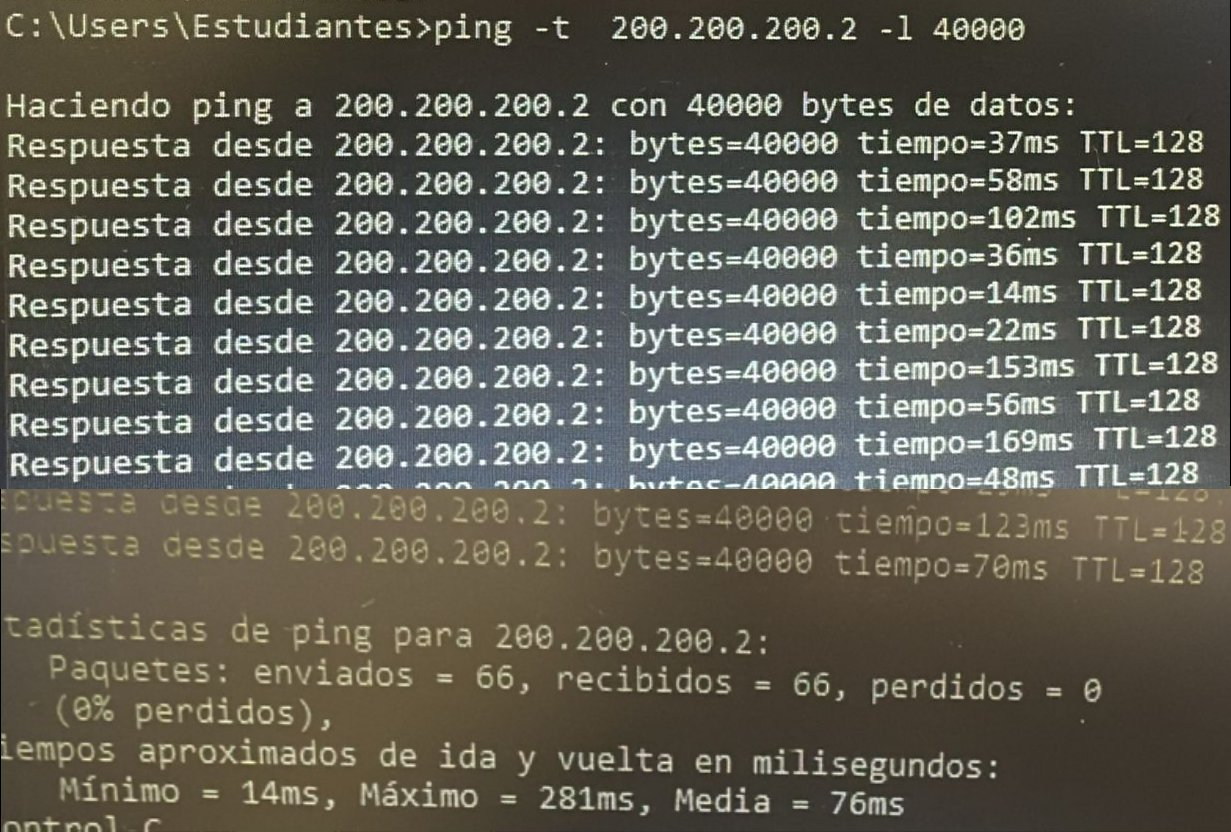
\includegraphics[width=\columnwidth]{punto1/p1_ping_wifi_lan_40k.jpeg}
        \caption{Ping Wifi - Lan, 40000}
        \label{fig:ping_wifi_lan_40k}
    \end{figure}

    \begin{figure}[H]
        \centering
        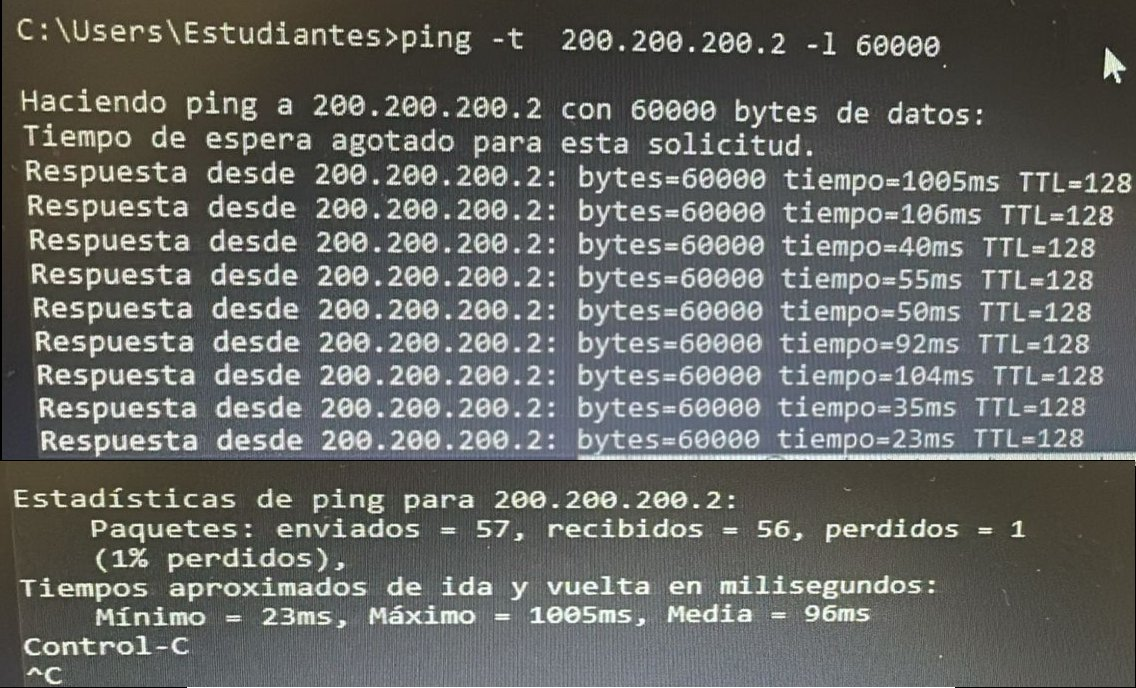
\includegraphics[width=\columnwidth]{punto1/p1_ping_wifi_lan_60k.jpeg}
        \caption{Ping Wifi - Lan, 60000}
        \label{fig:ping_wifi_lan_6k}
    \end{figure}


\subsubsection{Lan - Wifi}
Se hicieron prebas de ping Lan - Wifi con diferentes paquetes:
\begin{figure}[H]
    \centering
    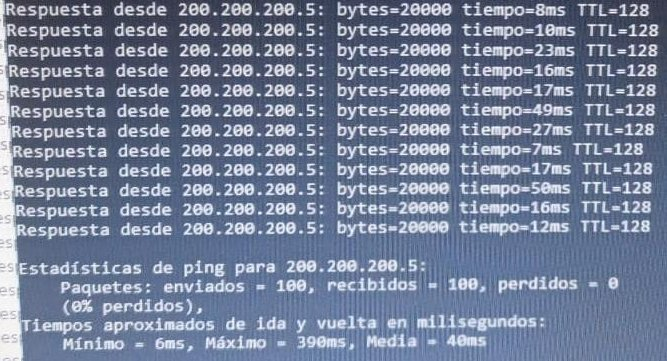
\includegraphics[width=\columnwidth]{punto1/p1_ping_lan_wifi_20k.jpeg}
    \caption{Ping Lan - Wifi, 20000}
    \label{fig:ping_lan_wifi_20k}
\end{figure}

\subsubsection{Wifi - Wifi}
Se hicieron prebas de ping Wifi - Wifi con diferentes paquetes:
\begin{figure}[H]
    \centering
    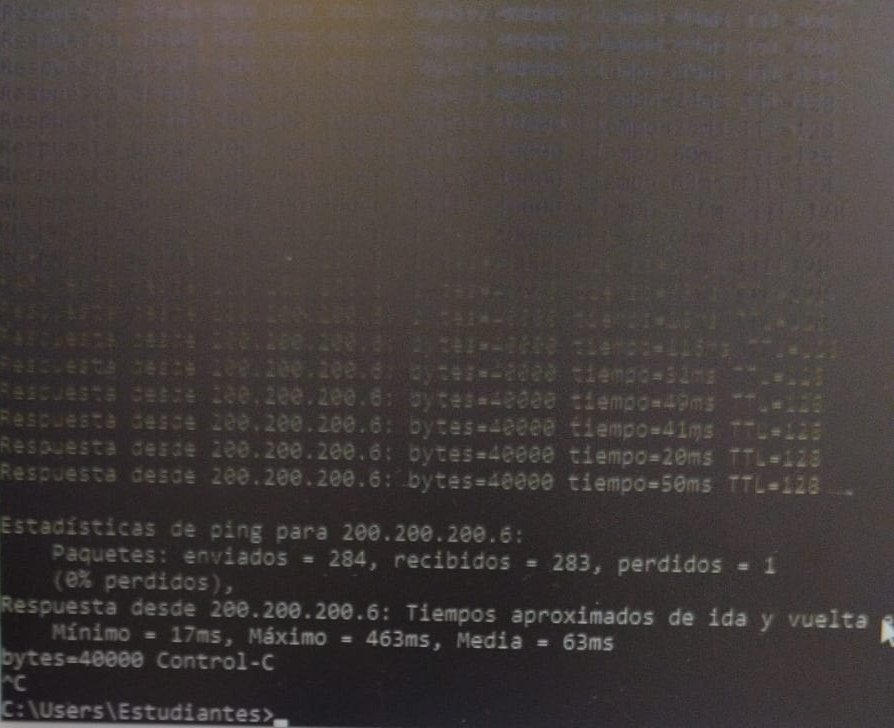
\includegraphics[width=0.8\columnwidth]{punto1/p1_ping_wifi_wifi_40k.jpeg}
    \caption{Ping Wifi - Wifi, 40000}
    \label{fig:ping_wifi_wifi_40k}
\end{figure}

\begin{figure}[H]
    \centering
    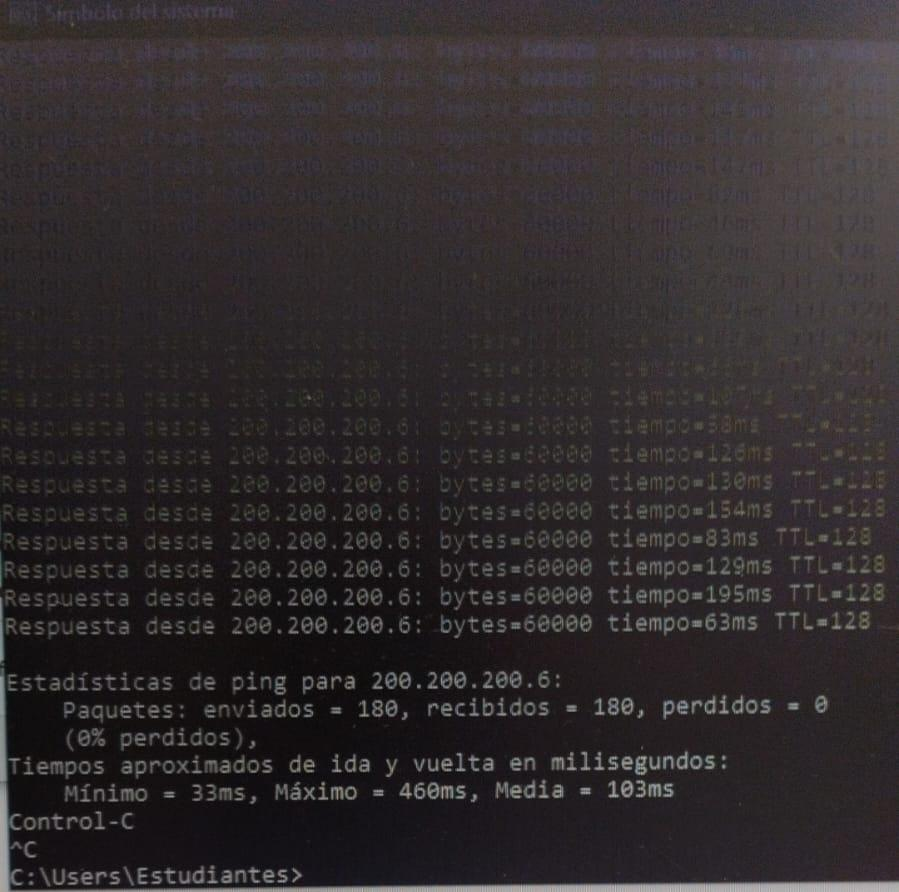
\includegraphics[width=0.8\columnwidth]{punto1/p1_ping_wifi_wifi_60k.jpeg}
    \caption{Ping Wifi - Wifi, 60000}
    \label{fig:ping_wifi_wifi_6k}
\end{figure}


%Haga una tabla y explique las diferencias que hay entre diferentes velocidades mínimo tres (3), entre las velocidades teóricas (ver tablas No. 1 y 2) y las velocidades obtenidas en la ejecución de los Pings.
% Nota 1: Hay que considerar las tablas No.1 y No. 2, con el fin de evaluar pertinentemente el estándar relacionado con las normas IEEE 802.3 y IEEE 802.11, ya que se presentan cambios con las velocidades y la técnica de modulación.
%

\begin{table}[H]
	\center
	\pgfplotstabletypeset[
		% Delimitador en el archivo
		% (puede ser comma, tab, space, etc.)
		col sep= ampersand,
		columns={T,t,D,P,V},
		% Nombres de columnas (ajústalos según tu archivo)
		columns/T/.style={string type,column name=Tamano$(bytes)$},
		columns/t/.style={string type,column name=$t(ms)$},
		columns/D/.style={string type,column name=Destino},
		columns/P/.style={string type,column name=P},
		columns/V/.style={string type,column name=$V(Mbps)$},
		every head row/.style={before row=\toprule, after row=\midrule},
		every last row/.style={after row=\bottomrule},
	]{punto1/tabla.dat}
	\caption{Tabla de velocidades}
	\label{t_1}
\end{table}

\begin{table}[H]
	\center
	\pgfplotstabletypeset[
		% Delimitador en el archivo
		% (puede ser comma, tab, space, etc.)
		col sep= semicolon,
		columns={O,P,V,T},
		% Nombres de columnas (ajústalos según tu archivo)
		columns/O/.style={string type,column name=O$(Mbps)$},
		columns/P/.style={string type,column name=P},
		columns/V/.style={string type,column name=$V(Mbps)$},
		columns/T/.style={string type,column name=$T(Mbps)$},
		every head row/.style={before row=\toprule, after row=\midrule},
		every last row/.style={after row=\bottomrule},
	]{punto1/p1_tab_2.dat}
	\caption{Diferencia, velocidad práctica y teórica}
	\label{t_2}
\end{table}

\begin{itemize}
	\item \small{O: Observable}
	\item \small{P: Protocolo}
	\item \small{V: Velocidad teórica probable (PHY)}
	\item \small{T: Throughput practico típico}
	\item \small{**: Si buena}
	\item \small{*: Ideal}
\end{itemize}
